\section{Auswertung}
\label{sec:Auswertung}
\subsection{Bestimmung des \texorpdfstring{\textsc{Planck}schen Wirkungsquantums $h$}{Planckschen Wirkungsquantums}}
\label{sec:Auswertung1}
Die Messwerte sind in Tabelle \ref{tab:messwerte} aufgetragen.
In Abbildungen \ref{fig:uidiagramm1} bis \ref{fig:uidiagramm2} sind die gemessenen Gegenspannungen $U$ gegen die Wurzel des Photostroms $I$ aufgetragen.
Die Parameter für die Ausgleichsgeraden werden nach den Formeln \eqref{eq:regress}
\begin{figure}[p]
\centering
Regression nach
\begin{subequations}
	\begin{equation}
		\Delta = N \sum{x^2} - {\biggl(\sum{x}\biggr)}^2,
	\end{equation}
	\begin{equation}
		a_{\text{Reg}} = \frac{N\sum{x\cdot y} - \sum{x} \cdot \sum{y}}{\Delta},
	\end{equation}
    \begin{equation}
		b_{\text{Reg}} = \frac{\sum{x^2} \cdot \sum{y} - \sum{x} \cdot \sum{x \cdot y}}{\Delta},
	\end{equation}
	\begin{equation}
		\sigma_{y} = \sqrt{\frac{\sum{(y - a_{\text{Reg}} \cdot x - b_{\text{Reg}})^2}}{N - 2}},
	\end{equation}
	\begin{equation}
		\sigma_{a} = \sigma_{y} \sqrt{\frac{N}{\Delta}},
	\end{equation}
	\begin{equation}
		\sigma_{b} = \sigma_{y} \sqrt{\frac{\sum{x^2}}{\Delta}}
	\end{equation}
	mit $x=x_\text{lin}=\frac{1}{T_m^2}$, $y=B$, $a_\text{Reg}=a_\text{lin}$, $b_\text{Reg}=b_\text{lin}$ und der Anzahl der Datenpaare N.
	\label{eq:regress}
\end{subequations}
\end{figure}
bestimmt.\\
Es ergeben sich die Fitparameter in Tabelle \ref{tab:abbfitwerte}.
Die y-Achsenabschnitte $b$ entsprechen der Grenzspannung $U$.
\begin{table}
	\centering
	\begin{tabular}{l S[table-format=3] S[table-format=1.4] S[table-format=1.3]}
		\toprule
		\multicolumn{2}{c}{Lichtspektrallinie} &\multicolumn{2}{c}{Fitparameter} \\
		{Farbe} & {Wellenlänge $\lambda$$/\:\si{\nano\meter}$} &{Steigung $a$/$\:\si{\volt\per{(\pico\ampere)\tothe{\sfrac{1}{2}}}}$} & {Abschnitt $b$$/\:\si{\volt}$}\\
		\midrule
			{rot} 			&640	&-0.25$\pm$0,01 		&0.77$\pm$0,02\\
			{gelb} 			&578	&-0.037$\pm$0,001  		&0.344$\pm$0,004\\
			{grün} 			&546	&-0.0271$\pm$0,0004 	&0.436$\pm$0,003\\
			{violett}		&435.8	&-0.0405$\pm$0,0008  	&0.911$\pm$0,007\\
			{ultraviolett} 	&366	&-0.084$\pm$0,002 		&1.47$\pm$0,02\\
		\bottomrule
	\end{tabular}
	\caption{Fitparameter der \texorpdfstring{Abbildungen \ref{fig:uidiagramm1} bis \ref{fig:uidiagramm2}}{U-I-Diagramme}}
	\label{tab:abbfitwerte}
\end{table}

Weiter werden die y-Achsenabschnitte $b$ der Fits gegen die Lichtfrequenz $\nu$ in Abbildung \ref{fig:unu} aufgetragen. 
Für die Umrechnung von Wellenlänge $\lambda$ und $\nu$ gilt
\begin{equation}
	c_0=\lambda\cdot\nu.
\end{equation}

Nach der Einsteinschen Formel \eqref{eq:einstein}
werden mithilfe der Linearisierung
\begin{align}
	%E_\text{kin.} &= e\cdot U = {h}\cdot{\nu} - {W_\text{K}}\\
	\underbrace{U}_{y_\text{Reg}} &= \underbrace{\frac{h}{e}}_{a_\text{Reg}}\cdot\underbrace{\nu}_{x_\text{Reg}} - \underbrace{\frac{W_\text{K}}{e}}_{b_\text{Reg}}\\
\end{align}
aus den Fitparametern das Plancksche Wirkungsquantum $h$ und die Austrittsarbeit $W_\text{K}$ bestimmt.

Es folgt
\begin{alignat}{3}
	\frac{h}{e}=\SI{3.4(6)e-15}{\weber} \quad&\text{und} \quad&&\frac{W_\text{K}}{e}= \SI{-1.4(4)}{\volt}.
\end{alignat}
\begin{figure}[H]
	\centering
	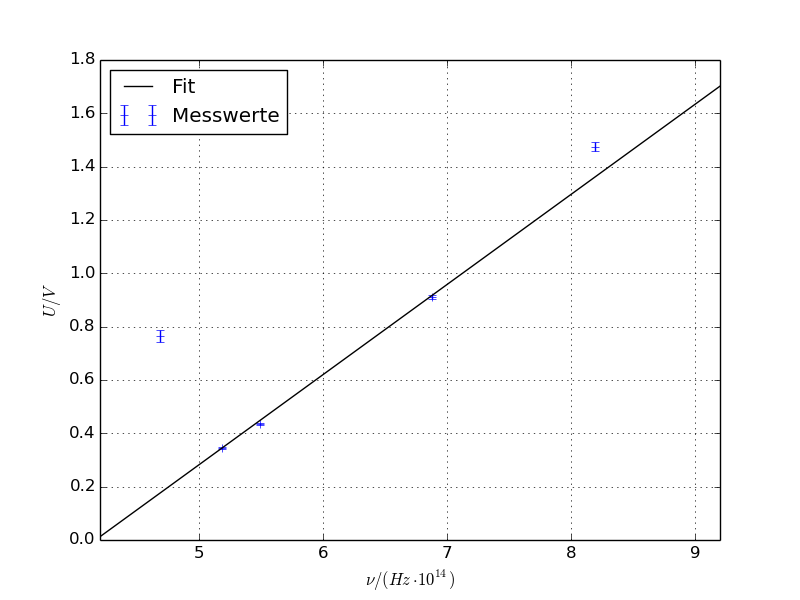
\includegraphics[width=\textwidth]{Bilder/unu_diag.png}
	\caption{Maximale Gegenspannung gegen die Lichtfrequenz. \cite{matplotlib}}
	\label{fig:unu}
\end{figure}
\newpage
\begin{figure}[p]
	\centering
	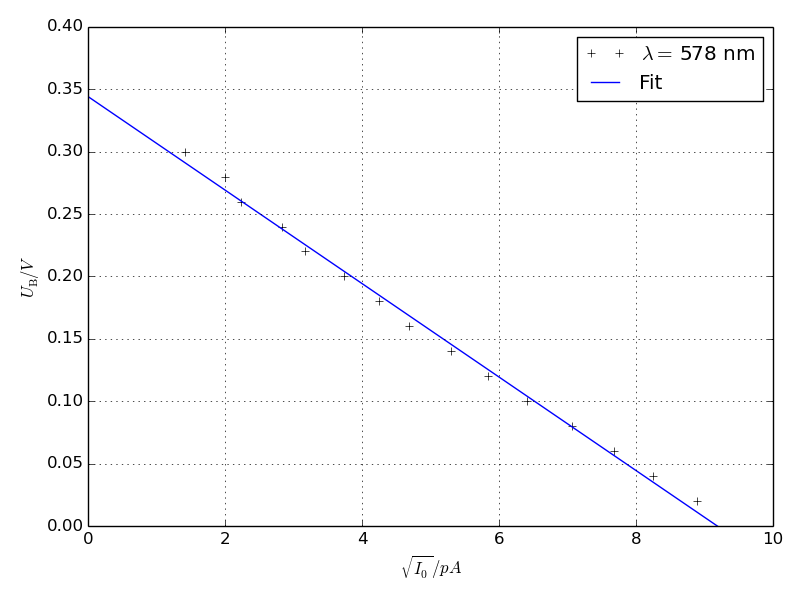
\includegraphics[width=0.8\textwidth]{Bilder/Fit_gelb.png}
	\caption{Gemessene Photostromstärken in Abhängigkeit von den Gegenspannungen, Messung bei gelber Spektrallinie.\cite{matplotlib}}
	\label{fig:uidiagramm1}
\end{figure}
\begin{figure}[p]
	\centering
	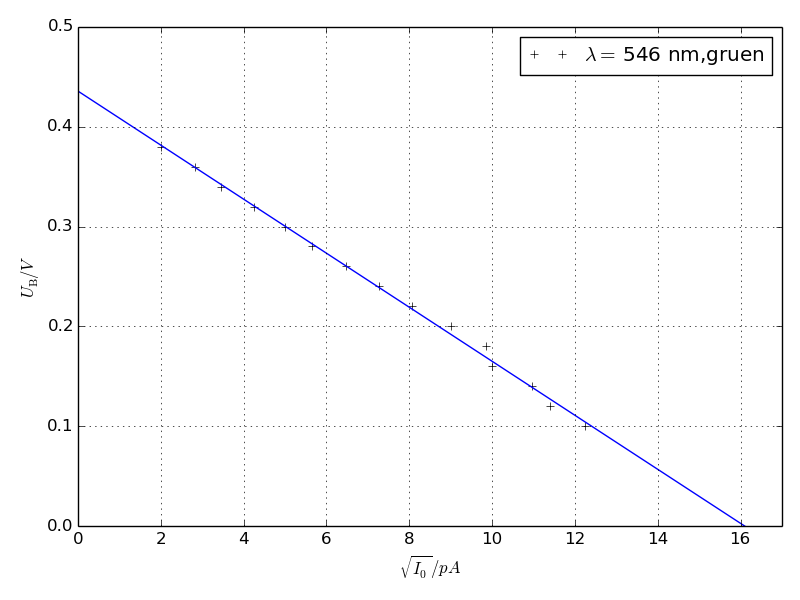
\includegraphics[width=0.8\textwidth]{Bilder/Fit_gruen.png}
	\caption{Gemessene Photostromstärken in Abhängigkeit von den Gegenspannungen, Messung bei grüner Spektrallinie.\cite{matplotlib}}
\end{figure}
\begin{figure}[p]
	\centering
	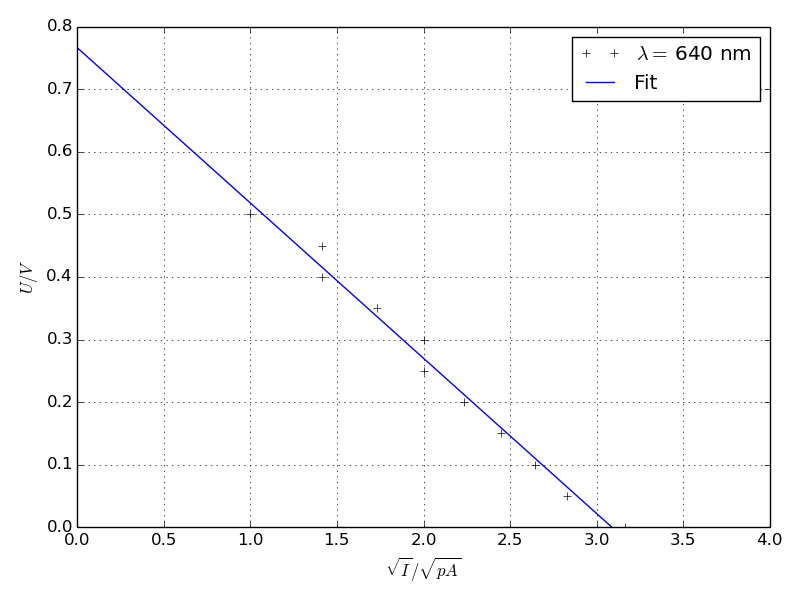
\includegraphics[width=0.8\textwidth]{Bilder/Fit_rot.png}
	\caption{Gemessene Photostromstärken in Abhängigkeit von den Gegenspannungen, Messung bei roter Spektrallinie.\cite{matplotlib}}
\end{figure}
\begin{figure}[p]
	\centering
	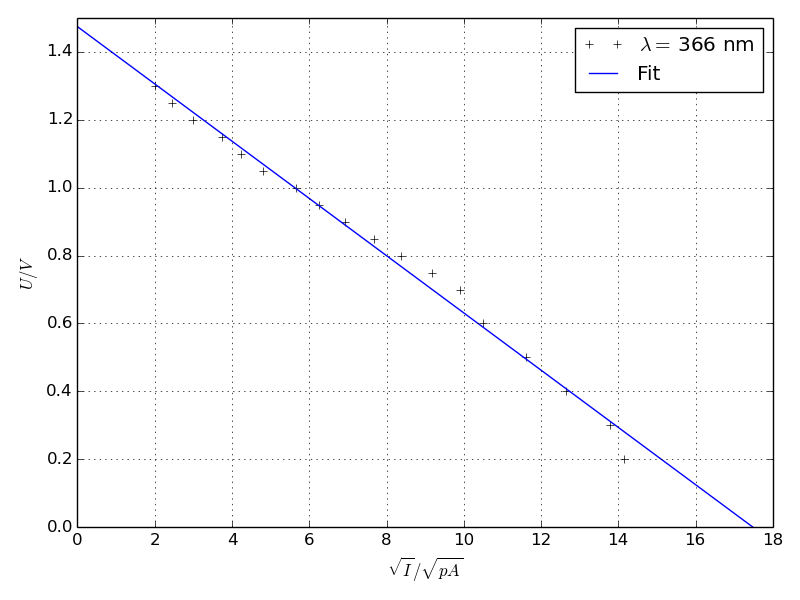
\includegraphics[width=0.8\textwidth]{Bilder/Fit_uv.png}
	\caption{Gemessene Photostromstärken in Abhängigkeit von den Gegenspannungen, Messung bei UV-Spektrallinie.\cite{matplotlib}}
\end{figure}
\begin{figure}[pt]
	\centering
	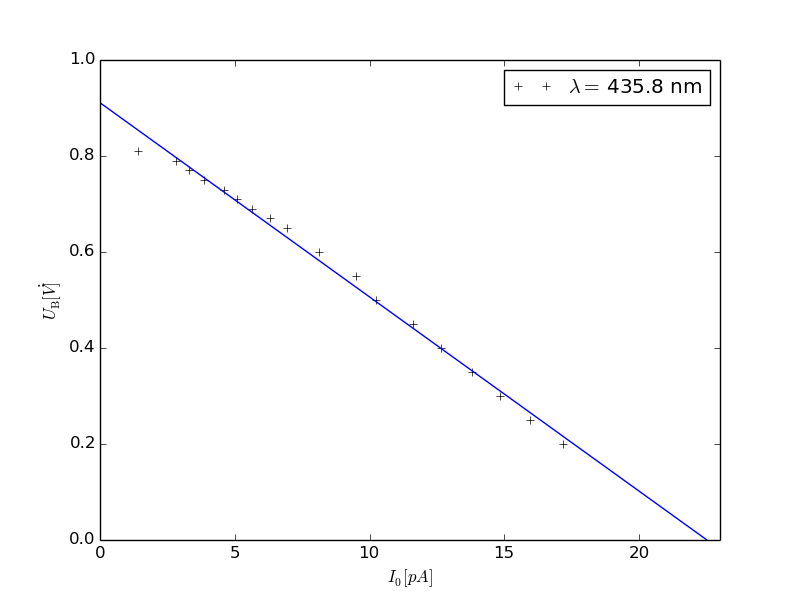
\includegraphics[width=\textwidth]{Bilder/Fit_violett.png}
	\caption{Gemessene Photostromstärken in Abhängigkeit von den Gegenspannungen, Messung bei violetter Spektrallinie.\cite{matplotlib}}
	\label{fig:uidiagramm2}
\end{figure}

\begin{landscape}
	\begin{minipage}[c][12cm][t]{0.3\textwidth}
		\centering
		\begin{tabular}{S[table-format=1.2] S[table-format=3.0]}
			\toprule
			\multicolumn{2}{c}{UV-Spektrallinie}\\ 
			\multicolumn{2}{c}{$\lambda=\SI{266.3}{\nano\meter}$}\\
			{$U_\text{B}/\:\si{\volt}$} & {$I_0/\:\si{\pico\ampere}$}\\	
			\midrule
				 0.20 & 200\\
				 0.30 & 190\\
				 0.40 & 160\\
				 0.50 & 135\\
				 0.60 & 110\\
				 0.70 &  98\\
				 0.75 &  84\\
				 0.80 &  70\\
				 0.85 &  59\\
				 0.90 &  48\\
				 0.95 &  39\\
				 1.00 &  32\\
				 1.05 &  23\\
				 1.10 &  18\\
				 1.15 &  14\\
				 1.20 &   9\\
				 1.25 &   6\\
				 1.30 &   4\\
				 1.345&   0\\
			\bottomrule
			\end{tabular}
	\end{minipage}
	\begin{minipage}[c][12cm][t]{0.3\textwidth}
		\centering
		\begin{tabular}{S[table-format=1.2] S[table-format=3.0]}
			\toprule
			\multicolumn{2}{c}{Violette Spektrallinie}\\ 
			\multicolumn{2}{c}{$\lambda=\SI{435.8}{\nano\meter}$}\\
			{$U_\text{B}/\:\si{\volt}$} & {$I_0/\:\si{\pico\ampere}$}\\	
			\midrule
				 0.20&	295\\
				 0.25&	255\\
				 0.30&	220\\
				 0.35&	190\\
				 0.40&	160\\
				 0.45&	135\\
				 0.50&	105\\
				 0.55&	 90\\
				 0.60&	 66\\
				 0.65&	 48\\
				 0.67&	 40\\
				 0.69&	 32\\
				 0.71&	 26\\
				 0.73&	 21\\
				 0.75&	 15\\
				 0.77&	 11\\
				 0.79&	  8\\
				 0.81&	  2\\
				 0.83&	  0\\
			\bottomrule
			\end{tabular}
	\end{minipage}
	\begin{minipage}[c][12cm][t]{0.3\textwidth}
		\centering
		\begin{tabular}{S[table-format=1.2] S[table-format=3.0]}
			\toprule
			\multicolumn{2}{c}{Grüne Spektrallinie}\\
			\multicolumn{2}{c}{$\lambda=\SI{546}{\nano\meter}$}\\
			{$U_\text{B}/\:\si{\volt}$} & {$I_0/\:\si{\pico\ampere}$}\\	
			\midrule
				0.10	&150\\	
				0.12	&130\\
				0.14	&120\\
				0.16	&100\\
				0.18	& 97\\
				0.20	& 81\\
				0.22	& 65\\
				0.24	& 53\\
				0.26 	& 42\\
				0.28	& 32\\
				0.30	& 25\\
				0.32	& 18\\
				0.34	& 12\\
				0.36	&  8\\
				0.38	&  4\\
				0.397	&  0\\
			\bottomrule
			\end{tabular}
	\end{minipage}
	\begin{minipage}[c][12cm][t]{0.3\textwidth}
		\centering
		\begin{tabular}{S[table-format=1.2] S[table-format=3.0]}
			\toprule
			\multicolumn{2}{c}{Gelbe Spektrallinie}\\
			\multicolumn{2}{c}{$\lambda=\SI{578}{\nano\meter}$}\\
			{$U_\text{B}/\:\si{\volt}$} & {$I_0/\:\si{\pico\ampere}$}\\	
			\midrule
				0.02	& 79\\
				0.04	& 68\\
				0.06	& 59\\
				0.08	& 50\\
				0.10	& 41\\
				0.12	& 34\\
				0.14	& 28\\
				0.16	& 22\\
				0.18	& 18\\
				0.20	& 14\\
				0.22	& 10\\
				0.24	& 8\\
				0.26	& 5\\
				0.28	& 4\\
				0.30	& 2\\
				0.32	& 0\\
			\bottomrule
			\end{tabular}
	\end{minipage}
	\begin{minipage}[c][12cm][t]{0.3\textwidth}
		\centering
		\begin{tabular}{S[table-format=1.2] S[table-format=3.0]}
			\toprule
			\multicolumn{2}{c}{Rote Spektrallinie}\\
			\multicolumn{2}{c}{$\lambda=\SI{640}{\nano\meter}$}\\
			{$U_\text{B}/\:\si{\volt}$} & {$I_0/\:\si{\pico\ampere}$}\\	
			\midrule
				0.00	&10\\
				0.05	& 8\\
				0.10	& 7\\
				0.15	& 6\\
				0.20	& 5\\
				0.25	& 4\\
				0.30	& 4\\
				0.35	& 3\\
				0.40	& 2\\
				0.45	& 2\\
				0.50	& 1\\
				0.506	& 0\\
			\bottomrule
			\end{tabular}
	\end{minipage}
\begin{table}[ht]
\caption{Die gemessenen Bremsspannungen \texorpdfstring{$U_\text{B}$}{U} und Photoströme \texorpdfstring{$I_0$}{I}in Abhängigkeit von der Wellenlänge \texorpdfstring{$\lambda$}{} des Lichtes.}
\label{tab:messwerte}
\end{table}
\end{landscape}
\subsection{Messung des \texorpdfstring{Photostromes $I$}{Photostromes} bei hohen \texorpdfstring{Spannungen $U$}{Spannungen}}
\label{sec:Auswertung2}
\begin{figure}[h]
	\centering
	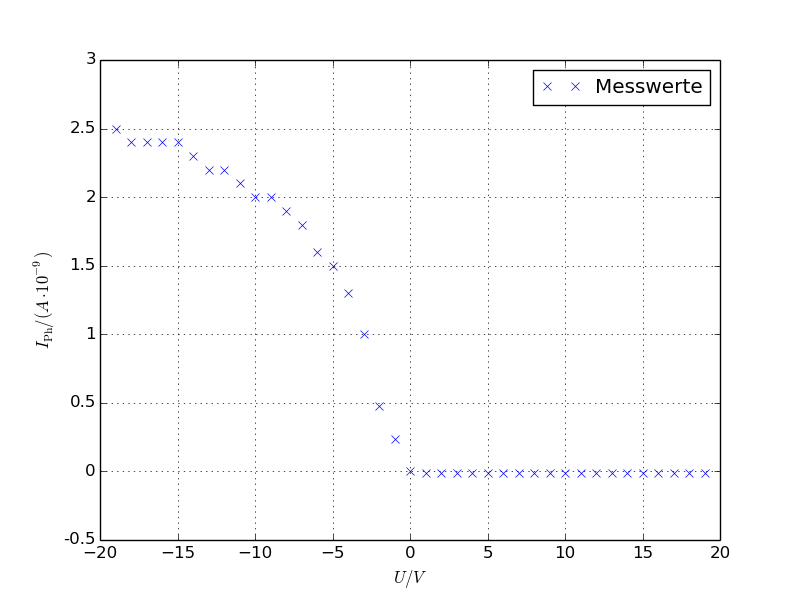
\includegraphics[width=\textwidth]{Bilder/messung2.png}
	\caption{Gemessener Photostrom in Abhängigkeit von der angelegten Spannung.\cite{matplotlib}}
	\label{fig:uidiagramm3}
\end{figure}


Wird keine Gegenspannung $U$ angelegt, so beträgt der Photostrom $I = \SI{80}{\pico\ampere}$.
In der vorhergegangen Messung wurde festgestellt, dass eine bremsende Spannung $U$ von etwa $\SI{0.34}{\volt}$ 
ausreichend ist, um den Photostrom $I$ vollständig zu unterdrücken.
Wird die Gegenspannung $U$ weit über diese Grenze angelegt, so stellt sich ein geringer, negativer Photostrom $I$ ein.
Dieser nimmt bereits für geringe Spannungen $U$ den Grenzwert $I=\SI{-0.01}{\nano\ampere}$ an und reagiert nicht auf weitere Erhöhung der Spannung $U$.

Wird eine negative Spannung $U$ angelegt, sodass die Photokathode negativ und die Anode positiv geladen ist, 
werden Photoelektronen beschleunigt.
Wird diese beschleunigende Spannung $U$ erhöht, so wächst der Photostrom $I$ an. 
Das Wachstum des Stromes $I$ ist für Spannungen $U$ bis etwa $\SI{5}{\volt}$ linear und geht für höhere Spannungen gegen einen Grenzwert von etwa $\SI{2.5}{\nano\ampere}$.